\section{The context}

Nowadays, web application's need are more sophisticated and demanding, such as 3D visualisation, audio and video,
games and so on. Efficiency and security are then important points that must be addressed, however JavaScript,
as the de facto standard language on the web, is not able to meet these requirements.

WebAssembly is a new language that is ``designed for efficient execution and compact representation of code
on modern processors including in a web browser'' \cite{wasm-w3c-announcement}, and strives to improve
both performance and power consumption.

\section{The Web}

\subsection{Basic structure}

The \textit{World Wide Web}, or more commonly \textit{Web}, is a collection of documents and other resources
that can be shared among various computers via the \textit{Internet}.

The resources shared are usually in the form of \textit{web pages}, documents whose structure is defined with HTML
(\textit{Hypertext Markup Language}) and whose styles are declared with CSS (\textit{Cascade Style Sheet}).
Other kind of resources include anything ranging from images, videos, audio, software and source code.

However, web pages are \textit{static} if they only use HTML and CSS, and cannot do much aside from showing content. A programming
language is hence needed to make the web \textit{dynamic}. Among all technologies and languages, nowadays
only JavaScript survives as the de facto standard language, used for both simple scripts and complex applications.

\subsection{JavaScript}
\label{sec:introduction-javascript}

\textit{JavaScript}, or \textit{JS} when abbreviated, is a high-level, dynamic, weakly typed programming language
that together with HTML and CSS is at the core of the World Wide Web. It conforms to the ECMAScript standard \cite{ecma-262}
and it can be both interpreted and \textit{just-in-time compiled}.

It was created in 1995 at Netscape and originally JavaScript engines were only run in web browsers, but there
are now runtime systems that allows the use of JavaScript directly on machines, such as \textit{Node.js} or \textit{Deno}.

Since JavaScript files are shared via the Web, there is the potential for authors to deliver
malicious scripts.
A common security vulnerability in the JavaScript world is \textit{cross-site scripting} (XSS), which is a violation of the
same-origin policy. These vulnerabilities occurs when an attacker is able to inject a malicious script in a target website
in order to, for example, access private information about the user.
Another vulnerability is \textit{cross-site request forgery} (CSRF), in which code on an attacker's website tricks the user's
browser into taking actions that the victim did not want to happen.

Sometimes hardware vulnerabilities can also be found - in 2019, the Spectre paper included a JavaScript implementation
alongside eBPF \cite{spectre}.

JavaScript is ill-equipped when it comes to performance-critical modern web pages - from this needs were born technologies
such as \textit{asm.js}, \textit{Native Client}, and eventually \textit{WebAssembly}.

\subsection{Web browsers and JavaScript runtimes}

A \textit{web browser} is a piece of software that enables users to access web pages shared on the World Wide Web, or a
local website. Browsers natively support the rendering of HTML and CSS, and feature an engine able to run JavaScript or, more commonly,
to just-in-time compile it in order to obtain more performance.

Browsers can also mitigate the risk provided by the common JavaScript vulnerabilities mentioned in Section \ref{sec:introduction-javascript}
by using two main methods - \textit{sandboxing}, so that JS isn't allowed to perform general-purpose
programming tasks like working directly with files\footnote{Although, there are APIs that can grant access to a ``virtual drive''
only when explicitly allowed by the user \cite{filesystem-mdn}, so access to the user's file system is not possible.},
and \textit{same-origin policy} constraints, in which scripts from one website have access to data from the same website but not others.

JavaScript can not only be executed on a browser, but also on so called ``back-end''
runtimes\footnote{Opposed to ``front-end'', which usually pertains to the browser}.
These runtimes offer custom libraries that enable JavaScript to access the file system, to make network requests,
spawn child processes and build complex applicatives, e.g.\ web servers.
Two notable runtimes are \textit{Node.js}\footnote{\url{https://nodejs.org/}} and \textit{Deno}\footnote{\url{https://deno.land}},
both open-source.
The first is built on top of Google's V8 engine, was initially released in 2009 and has a package manager called \textit{npm}
in order to manage its vast ecosystem of JS packages.
Deno, on the other hand, is a more modern runtime written in Rust, that includes support for TypeScript out of the box
and is \textit{secure by default}, since it blocks all file, network and environment access unless explicitely enabled.

\section{WebAssembly}

\subsection{Description and motivations}

\textit{WebAssembly} \cite{wasm-website} is a binary instruction format for a stack-based virtual machine.
It is designed to be a portable compilation target, so that different languages can be deployed on the web.
It was announced in 2015 and implemented by major browsers by 2017, and as of May 2022 is supported
by 93\% of all browsers\footnote{\url{https://caniuse.com/?search=WebAssembly}}.
WebAssembly main goals are to be \cite{bringing-the-web-up-to-speed-2017}:
\begin{itemize}
  \item \textit{Safe}, in particular to provide the same memory safety as a managed language;
  \item \textit{Fast}, by using ahead-of-time optimisations in a similar manner as native machine code;
  \item \textit{Portable}, since the web spans many device, architectures, operating systems and browsers;
  \item And finally \textit{compact}, because code is transmitted over the network and must reduce load times as much as possible.
\end{itemize}

There were previous attempt at solving the problem of having safe, fast and portable low-level code on the Web,
such as \textit{ActiveX}, \textit{Native Client} and \textit{asm.js}.

\textit{ActiveX} \cite{activex} was a Microsoft's technology for code-signing x86 binaries to run on the web, and relied only
on this signing. Hence, it achieved safety through a trust model, not through technical construction.
\textit{Native Client} \cite{native-client} introduced the first sandboxing technique for x86, ARM or MIPS machine code,
which was statically validated. Lastly, \textit{asm.js} \cite{asmjs} is a specialised subset of JavaScript, which is on of the target
languages of \textit{Emscripten} \cite{emscripten}, a compiler toolchain able to compile C/C++ applications in order to have them
run on browsers or on other JavaScript runtimes.

WebAssembly is available as a target for various languages, such as C/C++ with the aid of Emscripten, Rust,
AssemblyScript\footnote{A language with a syntax similar to TypeScript.}, Go, Kotlin, Swift and Zig.
The compiled binary can be then used from JavaScript on the web, or with Node.js or Deno, or even as a CLI application
with the aid of the \textit{WebAssembly System Interface} (see Section \ref*{sec:introduction-wasi}).

\subsection{Overview of the language}

Although WebAssembly is a binary code format, it can also be written with \textit{S-expressions}
in order to be more readable.
Each binary takes the form of a \textit{module}, which contains \textit{functions}, \textit{global} variables,
\textit{tables} and \textit{memories}. Each of these can be exported to be used in the embedder, and a module can also import functionalities.
While a module is a static representation of a program, an \textit{instance} is the dynamic one.
A module can be instantiated by the embedder (e.g.\ a JavaScript virtual machine).

\begin{code}[language=wasm, caption={Recursive factorial written in WebAssembly S-expressions}, label=lst:wasm-fact]
  (module
    (func $fact (param $x i64) (result i64)
      (if (result i64) (i64.eqz (local.get $x))
        (then (i64.const 1))
        (else
          (i64.mul
            (local.get $x)
            (call $fact
              (i64.sub (local.get $x) (i64.const 1)))))))
    (export "fact" (func $fact)))
\end{code}

WebAssembly is a typed language, but there are only four basic \textit{value types} - integers and IEEE 754 floating
point numbers, each in 32 and 64 bit variants. There are no distinction between signed and unsigned integers,
but instructions that depends on signedness are marked with an explicit suffix.

\textit{Functions} are typed, take a sequence of values as a parameter and returns another sequence of values.
They cannot be nested inside each other. The content of the call stack for execution are separate from the data
portion of the memory, and cannot be accessed directly by WebAssembly.
The code inside a function consists of a series of \textit{instructions} that modify an implicit operand stack,
either by declaring local variables or applying operations to the value already on the stack.
Functions can be called either \textit{directly} by using an index that identifies a function, or \textit{indirectly},
i.e.\ dynamically through a global \textit{table}. In this second case, only the function's type signature is validated.

WebAssembly has also support for \textit{traps} - in a similar manner to an exception, a trap aborts the current
computation, and control is given back to the embedder. For example, when embedded in JavaScript, a trap will
throw a JavaScript exception.

The main storage that WebAssembly uses is a \textit{linear memory} (or simply \textit{memory}), that is represented
by an array of bytes. Each module can defined no more than one memory, which can grow when needed with a unit size
of 64 KiB, a \textit{page}. This memory is separated by the call stack and by the memory dedicated to code.
Moreover, all pointers, when present, are translated into offsets in the linear memory, and all memory accesses are bound-checked.

Another main difference from other stack machines is that WebAssembly doesn't provide arbitrary jumps but
\textit{structured control flow}, so that the code can be validated in a single pass and prevent common control flow attacks.

\subsection{Problems with WebAssembly}

Since languages with manual memory management, such as C/C++, can be compiled into WebAssembly,
it is natural to ponder how memory vulnerabilities affect WebAssembly binaries.
In the original paper it is said that ``a buggy or exploited WebAssembly program can make a mess of the data in its own memory''
\cite{bringing-the-web-up-to-speed-2017}, in light of the fact that the call stack is not accessible by the program.

However, as shown in \cite{binary-security-wasm-2020}, even though WebAssembly strives for safety,
binaries can be still exploited with both traditional attacks,
such as buffer overflows, and attacks that aren't applicable in traditional native binaries, e.g.\ overwriting
string literals in memory.

The paper shows that it is possible to obtain a write primitive given a WebAssembly binary compiled from vulnerable C/C++ code,
by means of stack-based buffer overflows and heap metadata corruption, and it is possible to overwrite stack, heap and ``constant''
data, since the linear memory does not have a read-only section. It would be possible then, for example, to overwrite the name
of a file that was encoded as a string literal in the original program.

Another problem shown in the same paper is the redirection of indirect calls. Since WebAssembly allows indirect calls
to functions through a function table, an attacker could divert the execution by overwriting an integer in linear memory
that serves as an index into the table section. WebAssembly limits this ability with two mechanisms - not all functions
may appear in the table, but only those that can be indirectly called, and all functions call are type checked.
So, redirecting indirect calls is possible only within the class of functions with the same type.

Lastly, it is possible to enable remote code execution when including vulnerable WebAssembly in an application.
This is because functions that have different types in one language can be mapped onto functions with the same type
in WebAssembly. For example, a log functions that in C has the signature \texttt{void log(int)}, and a function such as
\texttt{void exec(const char* cmd)} both become functions with only one \texttt{i32} param in WebAssembly.
This enables the indirect diversion described in the previous paragraph if the two functions can be indirectly called.

\subsection{WASI - WebAssembly System Interface}
\label{sec:introduction-wasi}

The \textit{WebAssembly System Interface} (WASI) \cite{wasi} is a modular system interface for WebAssembly.
It focuses on security and portability so that WebAssembly binaries can be targeted by different languages
and then been safely run on different platforms.
Its API provides access to several OS-like features, such as file systems and Berkeley sockets.
The two languages that have good interoperability at the moment are Rust, where the compiler directly supports targeting WASM and WASI,
and C/C++, either through Emscripten or a custom prebuilt \textit{Clang} toolchain\footnote{\url{https://github.com/WebAssembly/wasi-sdk}}.

A binary that uses WASI can be run using a CLI runtime, such as \textit{Wasmtime} \cite{wasmtime} or \textit{Wasmer} \cite{wasmer},
or using a browser polyfill.
The approach taken for the sandboxing by these runtimes is based on a \textit{capability-based security model} \cite{wasmtime-security-sandboxing},
so that access to the file system must be explicitly given.
Moreover, writes to output streams are filtered when connected to a terminal in order to prevent control sequences
that may have side effects and confuse or mislead users.

The CLI runtimes have some particular features and properties:
\begin{itemize}
  \item It is possible to \textit{sandbox} entire directories by \textit{preopening} them, and eventually mapping them to custom paths
        , in order to have the files' descriptors available; it is not possible to escape this sandbox using the parent directory \texttt{..}
        or soft symlinks, but it is possible to escape using hard symlinks;
  \item The directory is the finest granularity available - once access is given to a specific directory, all files and subdirectories are
        visible, and there are no restrictions on permitted actions (reading, writing, deleting and creating files)\footnote{In C the binary can create files with specific user permissions on Linux, e.g.\ executable files.};
  \item When listing files in a directory, the only files that are visible are the ones that were already present at the preopening of the directory,
        but files added after the preopen can be read/written;
  \item Any change made to a file by any process is reflected in what the compiled WebAssembly binary is able to read;
  \item Environment variables are not accessible by default, but they must be explicitly declared;
  \item The WebAssembly memory is effectively sandboxed - the compiled cannot access memory outside its sandbox, otherwise a trap is raised;
  \item Not all ``classic'' functionality is available - when compiling C with the custom prebuilt toolchain,
        functions such as \texttt{system}, \texttt{execv} and \texttt{fexecve} are not available,
        so it is not possible to execute arbitrary commands or files;
  \item Fileless execution isn't feasible, since \texttt{memfd\_create} is not available due to the missing
        \texttt{sys/mman.h}\footnote{This library can be emulated, but \texttt{memfd\_create} is still not available}.
\end{itemize}

By using the \textit{wasm2c} tool available in the \textit{WebAssembly Binary Toolkit}\footnote{\url{https://github.com/WebAssembly/wabt}},
C code can be compiled into WebAssembly and then converted back to C.
This way, a traditional C program to use directly the functions made available from the original C library with an added sandbox
that allows code isolation. The sandboxed library cannot access locations outside its allocated memory without causing a trap,
halting the execution and giving back control to the embedder.
Similarly, the user C code cannot access the sandboxed memory directly, and if attempted it would result in a segmentation fault.

Lastly, as highlighted in \cite{wasmtime-security-sandboxing}, Spectre mitigations are not yet implemented, but are a topic of
ongoing research.

\subsection{WebAssembly as a fault isolation tool}

Since WebAssembly is \textit{sandboxed}, it is possible to isolate libraries that could be a frequent source of
vulnerabilities by compiling them to WebAssembly before their use.

An example is shown with the \textit{RLBox} project \cite{wasm-firefox-isolation-2020},
a framework that supports efficient sandboxing with modest performance overhead.
This project has been integrated into Firefox in order to sandbox the \texttt{libGraphite} font shaping library.

Even with the WASI interface it is possible to isolate a WebAssembly binary, since it is effectively \textit{sandboxed}
- all interactions with the embedding environment must be done through explicit exports and imports, and the memory is
bound checked at runtime, so that the WebAssembly program cannot access data outside its assigned memory, and the
embedder cannot access memory assigned to the WebAssembly code directly.

\section{Linux Security Modules}

The \textit{Linux Security Modules} (LSM) \cite{lsm-2002, kernel-lsm}
is a lightweight, general purpose, access control framework for the Linux Kernel.
It provides a mechanism for various security checks to be hooked by kernel extensions.
These extensions are not loadable kernel modules, but they can either be chosen at
compile-time via specific flags, such as \texttt{CONFIG\_DEFAULT\_SECURITY}, or overridden at boot-time.

The LSM is used primarily by \textit{Mandatory Access Control} (MAC) extensions to
provide a security policy. However, other extensions can be built with the LSM framework
in order to implement specific changes when they cannot be obtained with the functionality Linux itself.

Some projects that use LSM include:
\begin{itemize}
  \item \textit{SELinux} \cite{selinux}, i.e.\ \textit{Security Enhanced Linux}, that provides a mechanism for supporting advanced and fine-grained access control policies, as well as MAC;
  \item \textit{Smack} \cite{smack}, a kernel based implementation of MAC with simplicity as one of its primary goals;
  \item \textit{AppArmor} \cite{apparmor}, a MAC style security extension that implements a task centred policy.
\end{itemize}

\begin{figure}[ht]
  \centering
  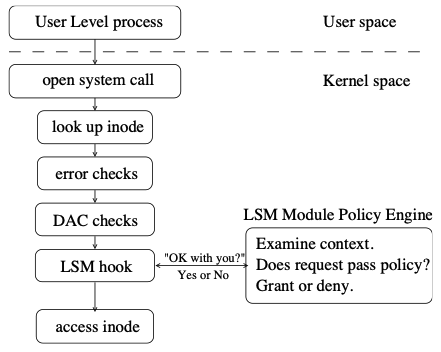
\includegraphics[width=0.6\linewidth]{lsm-hook-architecture.png}
  \caption{LSM Hook Architecture, from \cite{kernel-lsm}}
  \label{fig:lsm-hook-architecture}
\end{figure}

\subsection{Landlock}
\textit{Landlock} \cite{landlock-kernel, landlock-user-space} is a security feature available since Linux 5.13
that uses the LSM framework in order to provide scoped access control,
so that any process, even when unprivileged, can securely restrict itself.
This can help mitigate the security impact of bugs or unexpected/malicious behaviour
in user space applications.

Landlock employs the concept of \textit{rule}, which describes an action
on an object. An object is (currently) a file hierarchy, and actions are
defined with access rights, such as executing, reading or writing files, making
symbolic links and so on.
A set of rules is called a \textit{ruleset}, and it can restrict both the thread
using it and its future children, created either by spawning a new thread, as well
as using the \textit{fork} system call.

Notably, Landlock does not permits the definition of exceptions.
For example, suppose we have a directory \texttt{dir1}, which contains two files
\texttt{file1} and \texttt{file2}. We can define a ruleset that allows
reading and writing files for \texttt{dir1}.
However, if we then define another ruleset comprising only of read operations
for \texttt{file1}, the permissions specified for \texttt{dir1} are still
valid, so when a process restricts itself it is still able to write to \texttt{file1}.

In case of multiple consecutive self-restrictions, the result is the intersection
of all rulesets - if a process first restricts itself allowing all read and writing operations,
and then restricts itself again with only reading permissions, the result is equivalent
to a single restriction made with a ruleset that permits only reading operations.

Landlock can be used directly when writing C/C++ code in Linux thanks to the
\texttt{<linux/landlock.h>}\footnote{Examples of code available at \cite{landlock-user-space}}
header, or by using libraries that provide these binding to other languages,
such as \texttt{go-landlock}\footnote{\url{https://github.com/landlock-lsm/go-landlock}}
for Go and \texttt{rust-landlock}\footnote{\url{https://github.com/landlock-lsm/rust-landlock}} for Rust.

\subsection{eBPF}
\textit{eBPF} \cite{ebpf} is a virtual machine in the Linux Kernel that can run sandboxed programs
in a privileged context. It can be used to safely extend the capabilities of the kernel
without requiring to change kernel source code or load kernel modules.

Application developers can run eBPF programs in order to add additional capabilities at runtime,
and then the operating system guarantees safety and efficiency as if natively compiled
by using a Just-In-Time compiler.
These eBPF programs are event-driven and run when a certain hook point is passed. Some
predefined hooks include system calls, network events, and so on. If a hook does not exist,
it's possible to create custom kernel or user probes.

Unlike Landlock, eBPF makes it possible to define specific exception, e.g.\ denying
certain access rights on specific files while allowing them on the containing directory.
It also allows to specify whether a program has access to devices such as \texttt{terminal}
and \texttt{dev}.

Thanks to \texttt{BPFContain}\footnote{\url{https://github.com/willfindlay/bpfcontain-rs}}
it's also possible to run a container security daemon by leveraging eBPF.  In this case,
specific policies must be written for desired commands.